\documentclass[11pt]{article}
\newcommand{\name}{Jingbo Wang}

\usepackage[paper=letterpaper, margin=1in, headheight=13.6pt]{geometry}
\usepackage{fancyhdr}
\pagestyle{fancy}
\fancyhf{}
\rhead{\name{}}
\cfoot{Page \thepage}

\usepackage[parfill]{parskip}
\usepackage{amsmath}
\usepackage{graphicx}
\usepackage{fancyvrb}
\usepackage{upquote}

\newcommand{\problem}[1]{\vspace*{2ex}\textbf{Problem #1 ---} }
\newcommand{\answer}{\textit{Answer: }}

\begin{document}
\thispagestyle{empty}

\begin{center}
{\large CS 310}\\
Assignment 113\\
\today
\end{center}

\begin{flushright}
\name{}
\end{flushright}

The \texttt{pq.h} algorithm given in the assignment could Provide a priority 
queue based on an unsorted vector and the value in order. This is accomplished 
by \texttt{PriorityQueue} class.

The input size of the \texttt{pq.h} algorithm is $n$, defined on line 18 of 
the program.  

This algorithm has distinct best and worst cases.There are both best and worst 
cases run:

In function \texttt{void push(unsigned priority)}:
\begin{itemize}
    \item Line 30: a \texttt{push\_back} function call, 1 operation for each times, 
                   $n$ operations.
    \item Line 33: a \texttt{bubble\_up} function call, 1 operation for each times, 
                   $n$ operations.
\end{itemize}
In function \texttt{unsigned pop()}:
\begin{itemize}
    \item Line 43: an element assignment for \texttt{max\_value}, 2 operations for  
                   each times, $2n$ operations.
    \item Line 46: an element assignment for \texttt{array.at(0)}, 3 operations for  
                   each time, $3n$ operations.
    \item Line 49: a \texttt{pop\_back} function call, 1 operation for each times, 
                   $n$ operations. 
    \item Line 52: a \texttt{percolate\_down} function call, 1 operation for 
                   each times, $n$ operations.               
\end{itemize}
In function \texttt{bool is\_finish(size\_t position)} is used in function 
\texttt{void percolate\_down(size\_t position)}:

\begin{itemize}
    \item 161: an element assignment for \texttt{done}, 12 operations.
\end{itemize}

In function \texttt{void bubble\_up(size\_t position)} is Resurrection function, 
so we have:

\begin{itemize}
    \item Line 95: a \texttt{if} statement header call, 1 operation.
    \item Line 97: a \texttt{if} statement header call, 4 operations.
    \item Line 99: a \texttt{swap} function call, 2 operations.
    \item Line 104: an element assignment for \texttt{parent}, 3 operations.
\end{itemize}

For the function \texttt{void bubble\_up(size\_t position)} we have best case:

When the Line 95: \texttt{if} is false, the total operations: $1$ operation.

\begin{align*}
    T(n) &\geq 1 \\
         &\in \Omega(1)
\end{align*}

For the function \texttt{void bubble\_up(size\_t position)} we also have worse case:

All \texttt{if} statement are always true:

number of recursive calls($a$): 1

size of each recursive call($\frac{n}{b}$): $n/2$

Total operations($k$): $1 + 4 + 2 + 3 = 10$

$d$: 0

So, we have:

\begin{align*}
    T(n) & \geq 1 \times T(\frac{n}{2}) + 10n^0
\end{align*}

Because of $1 = 2^0$:

\begin{align*}
    T(n) & \leq 1 \times T(\frac{n}{2}) + 10n^0 \\
         & \in O(\lg n) 
\end{align*}

We run $n$ times for function 
\texttt{void bubble\_up(size\_t position)}, we have:

\begin{align*}
    T(n) &\geq 1 \\
         &\in \Omega(n) \\
    T(n) & \leq 10\lg n \\
         & \in O(\lg n) 
\end{align*}


In function \texttt{void percolate\_down(size\_t parent)}:
\begin{itemize}
    \item Line 118: a \texttt{if} statement header call, 
                    and includes a \texttt{is\_finish} function call, 17 operations. 
    \item Line 120--122: an element assignment for \texttt{position}, 
                           8 operations.
    \item Line 124: a \texttt{if} statement header call, 3 operations.
    \item Line 126: a \texttt{swap} function call, 2 operations.
    \item Line 128: an element assignment for \texttt{parent}, 3 operations.
    \item Line 133: a \texttt{swap} function call, 2 operations.
    \item Line 135: an element assignment for \texttt{parent}, 3 operations.
    \item Line 142: a \texttt{if} statement header call, 8 operations.
    \item Line 145: a \texttt{swap} function call, 2 operations.
\end{itemize}

For the function \texttt{void percolate\_down(size\_t parent)} we have best case:

When the Line 119: \texttt{if} is false, the total operations: $5$ operation.

\begin{align*}
    T(n) &\geq 5 \\
         &\in \Omega(1)
\end{align*}

For the function \texttt{void percolate\_down(size\_t position)} we also have worse case:

All \texttt{if} statement are always true:

number of recursive calls($a$): 1

size of each recursive call($\frac{n}{b}$): $n/2$

Total operations($k$): $17 + 5 + 8 + 3 + 2 + 3 + 2 + 3 + 8 + 2= 53$

$d$: 0

So, we have:

\begin{align*}
    T(n) & \leq 1 \times T(\frac{n}{2}) + 53n^0
\end{align*}

Because of $1 = 2^0$:

\begin{align*}
    T(n) & \leq 1 \times T(\frac{n}{2}) + 11n^0 \\
         & \in O(\lg n) 
\end{align*}

We run $n$ times for function \texttt{void percolate\_down(size\_t position)}, we have:

\begin{align*}
    T(n) &\geq 5 \\
         &\in \Omega(n) \\
    T(n) & \leq 53\lg n \\
         & \in O(\lg n) 
\end{align*}

For the \texttt{PriorityQueue} class call both \texttt{push} and \texttt{pop}
in the \texttt{analyze\_pq.cpp} running 
$n$ times, we have:

\begin{align*}
    T(n) & \geq n + n + 2n + 3n + n + n + n + 5n\\
         & \geq 15n \\
         & \in \Omega(n) \\
    T(n) & \leq n + n + 2n + 3n + n + n + 10n\lg n + 53n\lg n \\
         & \leq 63n\lg n + 9n \\
         & \in O(n\lg n) 
\end{align*}

The program was run with the command:

\begin{Verbatim}
for n in $(seq 100 10 10000)
do
    ./program $n
    ./program $n
    ./program $n
done 2> result.dat
\end{Verbatim}

in order to generate a set of points.  The resulting data were
plotted, giving the following.  Also plotted on the same axes are the
scaled standard functions $63n\lg n + 9n$ and $15n$ which illustrate 
that $63n\lg n + 9n$ that above the algorithm is worst case, and $15n$ below 
the algorithm is the best case.

\begin{center}
  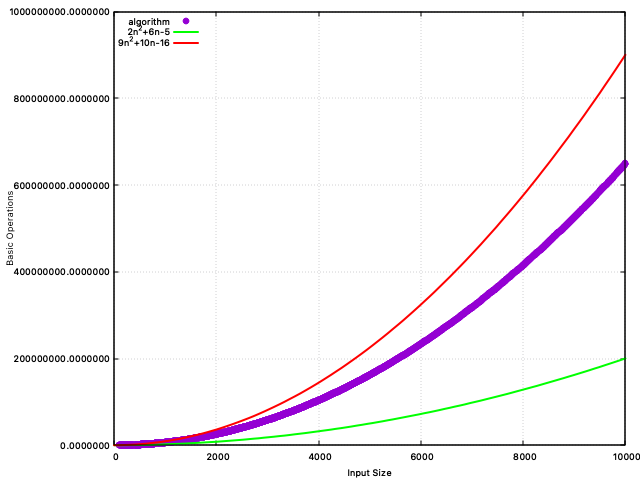
\includegraphics[width=0.7\textwidth]{analysis.png}
\end{center} 
We see that the plot confirms the theoretical analysis above.

It is same like we did in class.
\end{document}